% --------------------------------------------------------
% DEFINIÇÕES DO DOCUMENTO
% --------------------------------------------------------

\documentclass[
	% -- opções da classe memoir --
	12pt,				% tamanho da fonte
	openright,			% capítulos começam em pág ímpar (insere página vazia caso preciso)
	oneside,			% para impressão em verso e anverso. Oposto a twoside
	a4paper,			% tamanho do papel.
	% -- opções da classe abntex2 --
	%chapter=TITLE,		% títulos de capítulos convertidos em letras maiúsculas
	%section=TITLE,		% títulos de seções convertidos em letras maiúsculas
	%subsection=TITLE,	% títulos de subseções convertidos em letras maiúsculas
	%subsubsection=TITLE,% títulos de subsubseções convertidos em letras maiúsculas
	% -- opções do pacote babel --
	english,			% idioma adicional para hifenização
	french,				% idioma adicional para hifenização
	spanish,			% idioma adicional para hifenização
	brazil,				% o último idioma é o principal do documento
	]{lib/abntex2}


% --------------------------------------------------------
% PACOTES
% --------------------------------------------------------
\usepackage[section]{placeins}
\usepackage{cmap}				% Mapear caracteres especiais no PDF
\usepackage{lmodern}			% Usa a fonte Latin Modern
\usepackage[T1]{fontenc}		% Selecao de codigos de fonte.
\usepackage[utf8]{inputenc}		% Codificacao do documento (conversão automática dos acentos)
\usepackage{lastpage}			% Usado pela Ficha catalográfica
\usepackage{indentfirst}		% Indenta o primeiro parágrafo de cada seção.
\usepackage{color}				% Controle das cores
\usepackage{graphicx}			% Inclusão de gráficos
\usepackage{lipsum}				% para geração de dummy text

\let\printglossary\relax
\let\theglossary\relax
\let\endtheglossary\relax
\usepackage{lib/update-abntex}

\usepackage[brazilian,hyperpageref]{}	 % Paginas com as citações na bibl
\usepackage{microtype} 

\usepackage{silence}
%Disable all warnings issued by latex starting with "You have..."
\WarningFilter{latex}{You have requested package}
\usepackage[alf, abnt-etal-list=0 ]{lib/abntex2cite}	% Citações padrão ABNT
\usepackage[br]{lib/nicealgo}       % Pacote para criação de algoritmos
\usepackage{lib/customizacoes}      % Pacote de customizações do abntex2

\usepackage{listings}
\usepackage[normalem]{ulem} % Strikethrough package

% --------------------------------------------------------
% CONFIGURAÇÕES DE PACOTES
% --------------------------------------------------------
\definecolor{mygreen}{rgb}{0,0.6,0}
\definecolor{mygray}{rgb}{0.5,0.5,0.5}
\definecolor{mymauve}{rgb}{0.58,0,0.82}
\definecolor{darkgray}{rgb}{.4,.4,.4}
\definecolor{purple}{rgb}{0.65, 0.12, 0.82}

% Configurações do pacote listing
\renewcommand{\lstlistingname}{Código} %Mudança no caption do listing para Código
\renewcommand{\lstlistlistingname}{Lista de códigos} %Mudança no caption da lista de listings.

%Customize a bit the look
\lstset{
	backgroundcolor=\color{white}, % choose the background color; you must add \usepackage{color} or \usepackage{xcolor}
	basicstyle=\footnotesize, % the size of the fonts that are used for the code
	breakatwhitespace=false, % sets if automatic breaks should only happen at whitespace
	breaklines=true, % sets automatic line breaking
	captionpos=b, % sets the caption-position to bottom
	commentstyle=\color{mygreen}, % comment style
	deletekeywords={...}, % if you want to delete keywords from the given language
	escapeinside={\%*}{*)}, % if you want to add LaTeX within your code
	extendedchars=true, % lets you use non-ASCII characters; for 8-bits encodings only, does not work with UTF-8
	frame=single, % adds a frame around the code
	keepspaces=true, % keeps spaces in text, useful for keeping indentation of code (possibly needs columns=flexible)
	keywordstyle=\color{blue}, % keyword style
	% language=Octave, % the language of the code
	morekeywords={*,...}, % if you want to add more keywords to the set
	numbers=left, % where to put the line-numbers; possible values are (none, left, right)
	numbersep=5pt, % how far the line-numbers are from the code
	numberstyle=\tiny\color{mygray}, % the style that is used for the line-numbers
	rulecolor=\color{black}, % if not set, the frame-color may be changed on line-breaks within not-black text (e.g. comments (green here))
	showspaces=false, % show spaces everywhere adding particular underscores; it overrides 'showstringspaces'
	showstringspaces=false, % underline spaces within strings only
	showtabs=false, % show tabs within strings adding particular underscores
	stepnumber=1, % the step between two line-numbers. If it's 1, each line will be numbered
	stringstyle=\color{mymauve}, % string literal style
	tabsize=2, % sets default tabsize to 2 spaces
	title=\lstname % show the filename of files included with \lstinputlisting; also try caption instead of title
}

% define Javascript language
\lstdefinelanguage{JavaScript}{
	keywords={typeof, new, true, false, catch, function, return, null, catch, switch, var, if, in, while, do, else, case, break},
	keywordstyle=\color{blue}\bfseries,
	ndkeywords={class, export, boolean, throw, implements, import, this},
	ndkeywordstyle=\color{darkgray}\bfseries,
	identifierstyle=\color{black},
	sensitive=false,
	comment=[l]{//},
	morecomment=[s]{/*}{*/},
	commentstyle=\color{purple}\ttfamily,
	stringstyle=\color{red}\ttfamily,
	morestring=[b]',
	morestring=[b]",
	morestring=[b]`
}
 
\lstset{
	language=JavaScript,
	extendedchars=true,
	basicstyle=\footnotesize\ttfamily,
	showstringspaces=false,
	showspaces=false,
	numbers=left,
	numberstyle=\footnotesize,
	numbersep=9pt,
	tabsize=2,
	breaklines=true,
	showtabs=false,
	captionpos=b
}

% Configurações do pacote backref
\renewcommand{\familydefault}{\sfdefault}
% Usado sem a opção hyperpageref de backref
% \renewcommand{\backrefpagesname}{Citado na(s) página(s):~}
% Texto padrão antes do número das páginas
% \renewcommand{\backref}{}
% Define os textos da citação
% \renewcommand*{\backrefalt}[4]{
% 	\ifcase #1 %
% 		Nenhuma citação no texto.%
% 	\or
% 		Citado na página #2.%
% 	\else
% 		Citado #1 vezes nas páginas #2.%
% 	\fi}%


% --------------------------------------------------------
% INFORMAÇÕES DE DADOS PARA CAPA E FOLHA DE ROSTO
% --------------------------------------------------------

\titulo{Aplicativo para publicação e acompanhamento de alertas de segurança pública}
\autor{Bruno José Papa}
\local{Bauru}
\data{Março/2022}
\orientador{Profa. Dra. Roberta Spolon}
\instituicao{%
  Universidade Estadual Paulista ``Júlio de Mesquita Filho''
  \par
  Faculdade de Ciências
  \par
  Sistemas de Informação}
\tipotrabalho{Trabalho de Conclusão de Curso}
\preambulo{Trabalho de Conclusão de Curso do Curso de Bacharelado em Sistemas de Informação da Universidade Estadual Paulista ``Júlio de Mesquita Filho'', Faculdade de Ciências, Campus Bauru.}


% --------------------------------------------------------
% CONFIGURAÇÕES PARA O PDF FINAL
% --------------------------------------------------------

% alterando o aspecto da cor azul
\definecolor{blue}{RGB}{41,5,195}

% informações do PDF
\makeatletter
\hypersetup{
     	%pagebackref=true,
		pdftitle={\@title},
		pdfauthor={\@author},
    	pdfsubject={\imprimirpreambulo},
	    pdfcreator={LaTeX with abnTeX2},
		pdfkeywords={abnt}{latex}{abntex}{abntex2}{trabalho acadêmico},
		colorlinks=true,       		% false: boxed links; true: colored links
    	linkcolor=blue,          	% color of internal links
    	citecolor=blue,        		% color of links to bibliography
    	filecolor=magenta,      		% color of file links
		urlcolor=blue,
		bookmarksdepth=4
}
\makeatother


% ---
% Posiciona figuras e tabelas no topo da página quando adicionadas sozinhas
% em um página em branco. Ver https://github.com/abntex/abntex2/issues/170
\makeatletter
\setlength{\@fptop}{5pt} % Set distance from top of page to first float
\makeatother
% ---

% ---
% Possibilita criação de Quadros e Lista de quadros.
% Ver https://github.com/abntex/abntex2/issues/176
%
\newcommand{\quadroname}{Quadro}
\newcommand{\listofquadrosname}{Lista de quadros}

\newfloat[chapter]{quadro}{loq}{\quadroname}
\newlistof{listofquadros}{loq}{\listofquadrosname}
\newlistentry{quadro}{loq}{0}

% configurações para atender às regras da ABNT
\setfloatadjustment{quadro}{\centering}
\counterwithout{quadro}{chapter}
\renewcommand{\cftquadroname}{\quadroname\space} 
\renewcommand*{\cftquadroaftersnum}{\hfill--\hfill}

\setfloatlocations{quadro}{hbtp}
% ---


% --------------------------------------------------------
% ESPAÇAMENTOS ENTRE LINHAS E PARÁGRAFOS
% --------------------------------------------------------

% O tamanho do parágrafo é dado por:
\setlength{\parindent}{1.3cm}

% Controle do espaçamento entre um parágrafo e outro:
\setlength{\parskip}{0.2cm}


% --------------------------------------------------------
% COMPILANDO O ÍNDICE
% ---------------------------------------------------
\makeindex
% ---
 
% ---
% GLOSSARIO
% ---
\makeglossaries
% ---
% Exemplo de configurações do glossairo
\renewcommand*{\glsseeformat}[3][\seename]{\textit{#1}  
 \glsseelist{#2}}
% ---
 
% --------------------------------------------------------
% INÍCIO DO DOCUMENTO
% --------------------------------------------------------

\begin{document}

% Seleciona o idioma do documento (conforme pacotes do babel)
\selectlanguage{brazil}

% Retira espaço extra obsoleto entre as frases.
\frenchspacing


% --------------------------------------------------------
% ELEMENTOS PRÉ-TEXTUAIS
% --------------------------------------------------------

% Capa
\imprimircapa

% Folha de rosto
% (o * indica que haverá a ficha bibliográfica)
\imprimirfolhaderosto*

\begin{fichacatalografica}
	\sffamily
	\vspace*{\fill}					% Posição vertical
	\begin{center}					% Minipage Centralizado
		\fbox{\begin{minipage}[c][7.5cm]{12.5cm}		% Largura
			\small
			\imprimirautor
			\hspace{0.5cm} \imprimirtitulo  / \imprimirautor. --
			\imprimirlocal, \imprimirdata-
			\hspace{0.5cm} \pageref{LastPage} p. : il. (algumas color.) ; 30 cm.\\
			\hspace{0.5cm} \imprimirorientadorRotulo~\imprimirorientador\\
			\hspace{0.5cm}
			\parbox[t]{\textwidth}{\imprimirtipotrabalho~--~\imprimirinstituicao,
				\imprimirdata.}
			\end{minipage}}
	\end{center}
\end{fichacatalografica}

\begin{folhadeaprovacao}
	\begin{center}
		{\ABNTEXchapterfont\large\imprimirautor}
		\vspace*{\fill}\vspace*{\fill}
		\begin{center}
			\ABNTEXchapterfont\bfseries\Large\imprimirtitulo
		\end{center}
		\vspace*{\fill}
		\hspace{.45\textwidth}
		\begin{minipage}{.5\textwidth}
			\imprimirpreambulo
		\end{minipage}%
		\vspace*{\fill}
	\end{center}
	\center Banca Examinadora
	\assinatura{\textbf{\imprimirorientador} \\ Orientadora\\
		Departamento de Computação \\
		Faculdade de Ciências \\
	Universidade Estadual Paulista "Júlio de Mesquita Filho"}
	\assinatura{\textbf{Prof. Dr. José Remo Ferreira Brega} \\
		Departamento de Computação \\
		Faculdade de Ciências \\
	Universidade Estadual Paulista "Júlio de Mesquita Filho"}
	\assinatura{\textbf{Profa. Dra. Márcia A. Zanoli Meira e Silva} \\
		Departamento de Computação \\
		Faculdade de Ciências \\
	Universidade Estadual Paulista "Júlio de Mesquita Filho"}
	\begin{center}
		\vspace*{0.5cm}
		\par
		{Bauru, \_\_\_\_\_ de \_\_\_\_\_\_\_\_\_\_\_ de \_\_\_\_.}
		\vspace*{1cm}
	\end{center}
\end{folhadeaprovacao}

% \begin{dedicatoria}
% 	\vspace*{\fill}
% 	\begin{flushright}
% 		\textit{Espaço destinado à dedicátoria do texto.} 
% 	\end{flushright}
% \end{dedicatoria}

% \begin{agradecimentos}
% 	Espaço destinado aos agradecimentos.
% \end{agradecimentos}

% \begin{epigrafe}
% 	\vspace*{\fill}
% 	\begin{flushright}
% 		\textit{Espaço destinado à epígrafe.}\\
% 		Não esquecer autor
% 	\end{flushright}
% \end{epigrafe}


% --------------------------------------------------------
% RESUMOS
% --------------------------------------------------------

\setlength{\absparsep}{18pt} % ajusta o espaçamento dos parágrafos do resumo

% resumo em português
\begin{resumo}
	O presente trabalho apresenta a análise, projeto, implementação e avaliação de uma aplicação móvel para a publicação e o acompanhamento de alertas relacionados à segurança pública no Brasil, o qual é capaz de manter as pessoas conscientes de eventuais perigos nos seus arredores em tempo real. Essas informações fornecidas pelas comunidades locais podem ser cruciais para que as pessoas busquem se proteger e proteger uns aos outros. É exposto que a tecnologia, aliada com a colaboração entre usuários pela internet, pode também ser uma importante ferramenta de segurança. As principais funcionalidades do aplicativo desenvolvido são: rastreamento da localização do usuário, publicação de alertas com suporte ao envio de imagens e vídeos, e o disparo de notificações baseados em localização. É importante ressaltar que este trabalhado não estimula que a justiça seja feita com as próprias mãos, uma vez que isso é resposabilidade dos orgãos públicos locais.
	\\
	\textbf{Palavras-chave:} Aplicação móvel, Sistema colaborativo, Engenharia de software
\end{resumo}

\begin{resumo}[Abstract]
	\begin{otherlanguage*}{english}
		The current project presents the analyze, design, implementation and evaluation of a mobile application for the publication and monitoring of alerts related to public safety in Brazil, which is capable of keeping people aware of possible dangers in their surroundings in real time. This informations provided by local communities can be crucial for people to seek to protect themselves and each other. It is exposed that the technology, combined with collaboration between users over the internet, can also be an important security tool. The main features of the developed application are: user's location tracking, publishing alerts with images and videos uploads suports, and triggering location-based notifications. It is important to emphasize that this work does not encourage justice to be done with their own hands, since this is the responsibility of local public bodies.
		\\
		\textbf{Keywords:} Mobile application, Collaborative system, Software engineering.
	\end{otherlanguage*}
\end{resumo}

% --------------------------------------------------------
% LISTA DE ILUSTRAÇÕES
% --------------------------------------------------------
\pdfbookmark[0]{\listfigurename}{lof}
\listoffigures*
\cleardoublepage

% --------------------------------------------------------
% LISTA DE QUADROS
% --------------------------------------------------------
% \pdfbookmark[0]{\listofquadrosname}{loq}
% \listofquadros*
% \cleardoublepage
% ---

% --------------------------------------------------------
% LISTA DE TABELAS
% --------------------------------------------------------
% \pdfbookmark[0]{\listtablename}{lot}
% \listoftables*
% \cleardoublepage

% --------------------------------------------------------
% LISTA DE ABREVIATURAS E SIGLAS
% ---
\begin{siglas}
	\item[API] \emph{Application Programming Interface}
	\item[AWS] \emph{Amazon Web Services}
	\item[DTO] \emph{Data Transfer Object}
	\item[HTTP] \emph{Hypertext Transfer Protocol}
	\item[IaC] \emph{Infrastructure as Code}
	\item[ORM] \emph{Object-Relational Mapping}
	\item[RDS] \emph{Relational Database Service }
	\item[REST] \emph{Representational State Transfer}
	\item[SDK] \emph{Software Development Kit}
	\item[S3] \emph{Simple Static Storage}
\end{siglas}
% --------------------------------------------------------

% --------------------------------------------------------
% SUMÁRIO
% --------------------------------------------------------

% inserir o sumario
\pdfbookmark[0]{\contentsname}{toc}
\tableofcontents*
\cleardoublepage

% --------------------------------------------------------
% ELEMENTOS TEXTUAIS
% --------------------------------------------------------

\pagestyle{simple}

\chapter{Introdução}
\label{c.introducao}

Os sistemas colaborativos revolucionaram a forma como as pessoas se relacionam. Eles permitem com que uma tarefa complexa seja dividida entre pequenas tarefas simples distribuídas entre várias pessoas, eles rompem as barreiras físicas para a viabilizar a conexão de pessoas até então desconhecidas entre si, eles possibilitam, através de um efeito de rede, a construção de um senso de comunidade, que é autossuficiente e orgânico.

Dentre esses sistemas, existem os sistemas conectadores, que são plataformas que fornecem toda a infraestrutura necessária para unir pessoas que são provedoras de um serviço às pessoas que são as consumidoras desse serviço, como aplicativos de transporte que permitem a busca por motoristas baseada na localização. Existem também os sistemas de colaboração em massa, do inglês \emph{crowdsourcing}, que se beneficia ainda mais do poder da colaboração entre milhões de pessoas, como, por exemplo, o Wikipedia ~\cite{wikipedia}, a maior enciclopédia livre da internet.

A tecnologia, aliada à colaboração entre usuários, pode também ser uma importante ferramenta de segurança. Um grande exemplo de sucesso é aplicativo Waze ~\cite{waze}, onde o usuário pode contribuir com alertas de acidentes de trânsito e com informações de rotas que estão congestionadas. Há, portanto, uma relação ganha-ganha para todas as partes envolvidas.

\section{Motivação}
\label{s.motivacao}
% “Por que o problema tratado é relevante?” 

O Brasil é um país onde as pessoas, sobretudo aquelas que residem em grandes centros urbanos, vivem constantemente com uma sensação de insegurança em decorrência do medo de assaltos, furtos, roubos e crimes em geral que, apesar de ser dever do Estado garantir a segurança pública, muitas vezes o tempo de resposta é muito alto. Somado à isso, catástrofes naturais são cada vez mais comuns em virtude do aquecimento global.

\section{Solução}
\label{s.solucao}
% “O que será desenvolvido e como isto será utilizado para resolver o problema em questão?” 

Tendo em vista a tendência do uso de sistemas facilitadores para a economia colaborativa, é apresentado neste trabalho uma solução para emponderar as comunidades locais a se protegerem e proteger uns aos outros usando a tecnologia como uma ferramenta de segurança. Por meio de um aplicativo móvel de celular, pessoas poderiam ser alertadas e alertar outras pessoas próximas sobre a ocorrência de crimes, tiroteios, incêndios, emergências, protestos, ruas interditadas, catástrofes naturais, entre outros incidentes que coloquem em risco a segurança das pessoas.

\section{Desafios}
\label{s.desafios}
% “Quais serão as maiores dificuldades para alcançar a solução desejada?

A solução desejada possui desafios técnicos, como a implementação de um sistema de notificações e um mecanismo de rastreamento em tempo real da localização do usuário.

Além disso, a própria solução trás consigo muitos desafios. Qualquer dado que vem do usuário deve ser motivo de preocupação, é preferível que eles sejam padronizados, validados, ou até sanitizados, se for o caso. A veracidade da informação fornecida por eles também é um risco, o usuário pode, com má intenção ou por engano, cometer injustiças sociais como calúnia, difamação, injúria racial, ou adicionar conteúdo explícito ou depreceativo. Portanto, além dos desafios técnicos, o maior desafio é o de oferecer formas para tentar mitigar esses problemas de confiança que são intrínsicos ao ser humano.

% TODO: O final da introdução deve incluir uma descrição de como o documento está estruturado (um parágrafo para indicar o conteúdo de cada seção).
\chapter{Soluções existentes e objetivos da proposta}

% https://capozzielli.gdigital.com.br/usuario/

% https://www.techtudo.com.br/tudo-sobre/bo-coletivo.html
% No Brasil, o aplicativo \emph{BO coletivo} permite com que os usuários colaborem com um mapeamento coletivo de assaltos, furtos, roubos e sequestros. Porém, ele é útil apenas para consultas posteriores, não oferecendo mecanismos para ações preventivadas em tempo real, e também, em relação à usabilidade, o aplicativo não permite a navegação pelo mapa ao digitar uma região desejada.

\section{Soluções existentes}

% - Deve-se fazer uma pesquisa de soluções existentes para o mesmo problema que deseja resolver.
% - As soluções pesquisadas devem ser descritas com profundidade suficiente para que fique caracterizada sua competência em resolver o problema em questão, bem como seus aspectos positivos e negativos.

\subsection{Citizen}

O aplicativo \emph{Citizen} ~\cite{citizen}, desenvolvido pela \emph{sp0n, Inc.}, foi lançado originalmente em 2016 com o nome de \emph{Vigilante} em alguns grandes centros dos Estados Unidos. Em junho de 2020, ele possuía cerca de 5 milhões de usuários ativos. Seu sucesso vem da sua robustez, usabilidade, velocidade e praticidade. Entre as principais funcionalidades destacam-se o envio de alertas de segurança baseado na localização em tempo real, o acompanhamento pelos usuários dos alertas que estão em andamento, a transmissão de vídeos ao vivo e a possibilidade de adicionar comentários. As suas notificações já ajudaram pessoas à evacuarem de prédios em chamas e ônibus escolares à escaparem de ataques terroristas. 

A empresa dona do aplicativo, \emph{sp0n, Inc}, possui antenas de rádio nas cidades suportadas para que as chamadas telefônicas da polícia local sejam monitadoras, permitindo com que operadores especializados da empresa as filtrem e publiquem alertas no aplicativo. Em razão disso, o aplicativo \emph{Citizen} tem sua atuação dependente dos orgãos públicos. Em agosto de 2020, ele atuava em apenas 60 cidades dos Estados Unidos.

A Figura~\ref{f.citizen} mostra algumas das principais telas do aplicativo.

\begin{figure}[h]
	\caption{\small Telas do aplicativo Citizen.}
	\centering
	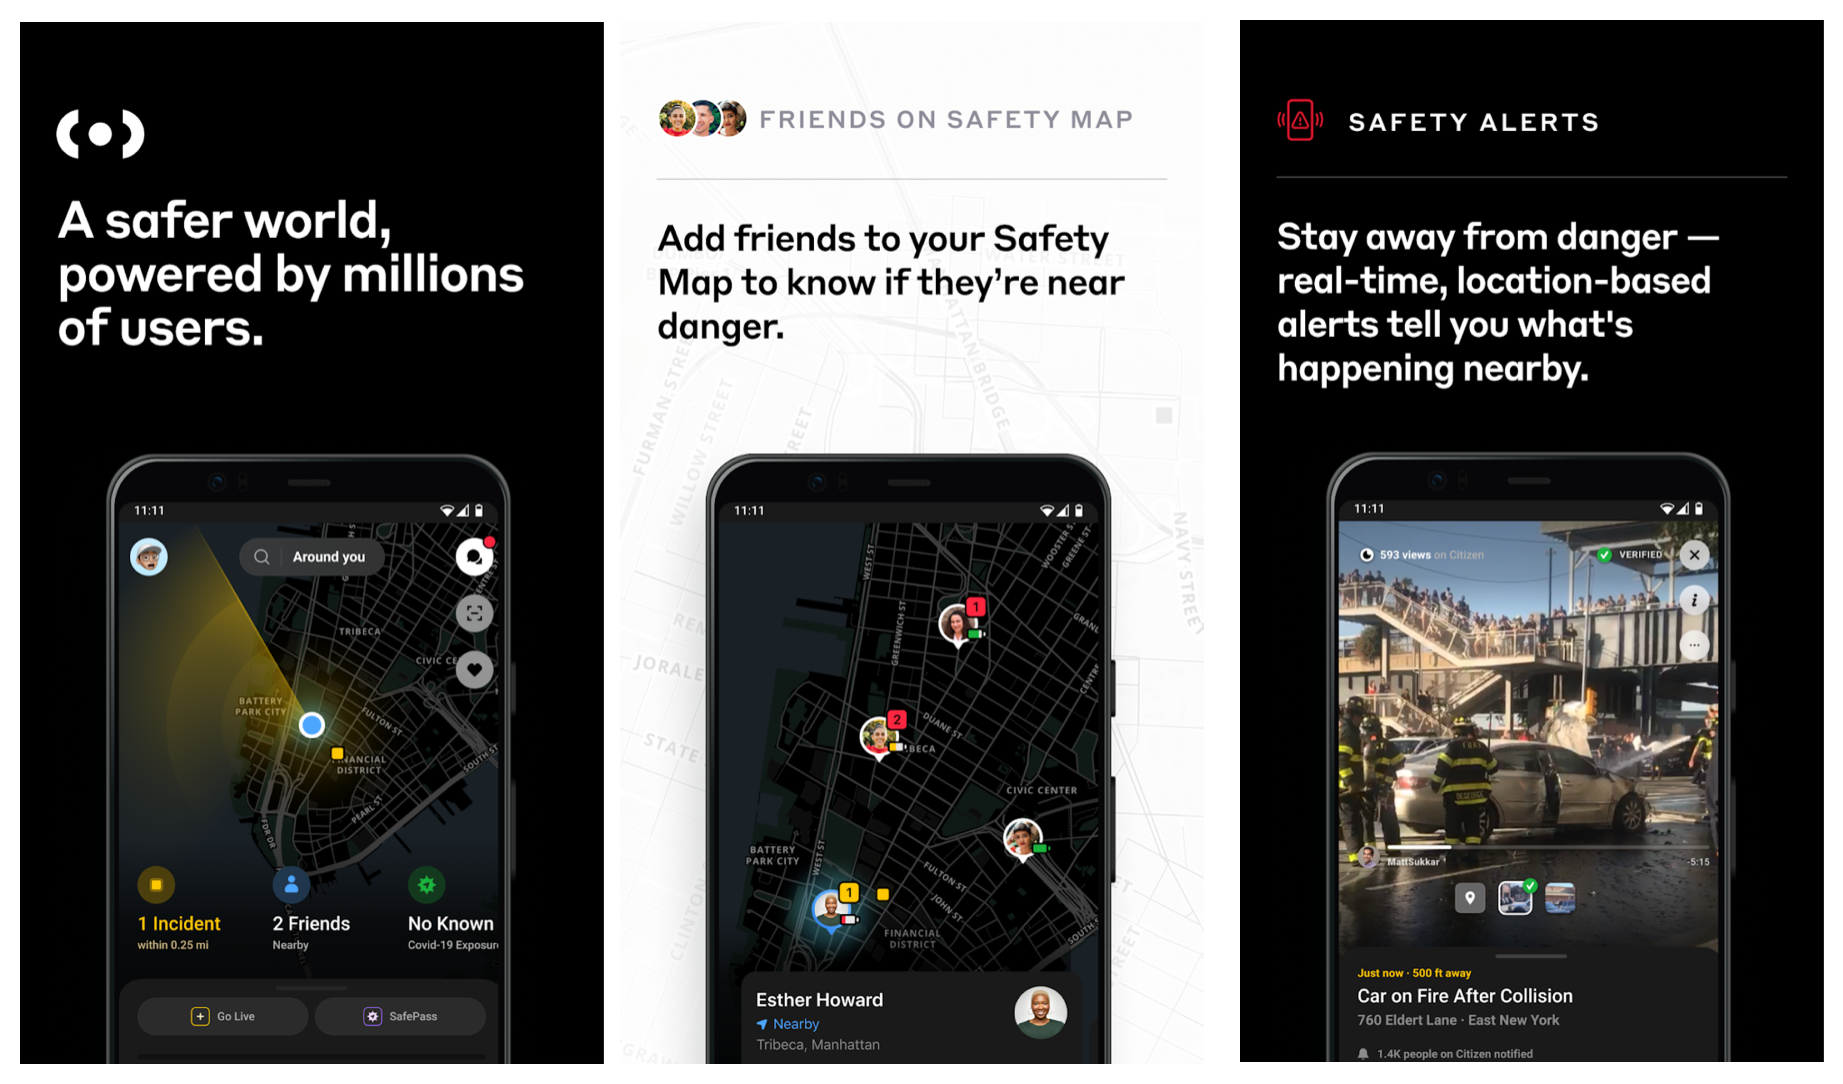
\includegraphics[width=\textwidth]{./images/citizen.png}
	\label{f.citizen}
	\legend{\small Fonte: Google Play.}
\end{figure}

\subsection{SP+ segura}

O aplicativo \emph{SP+ segura} ~\cite{sp-mais-segura} foi lançado pela Secretaria Municipal de Segurança Urbana de São Paulo em novembro de 2017. Com mais de 50 mil usuários, o aplicativo permite com que pessoas informem e sejam informadas de alertas em tempo real sobre episódios de risco em que pessoas se encontram ou presenciam. 

Ele oferece a opção de ligar para o orgão público responsável para acioná-lo quando for necessário. Porém, ele não oferece interação de chat entre usuários para eventuais discussões, e não suporta o envio de vídeos. Além disso, conta com muitas avaliações negativas na loja de aplicativos pelos usuários, com criticas à baixa qualidade.

A Figura~\ref{f.sp-mais-segura} mostra as principais telas do aplicativo.

\begin{figure}[h]
	\caption{\small Telas do aplicativo SP+ segura.}
	\centering
	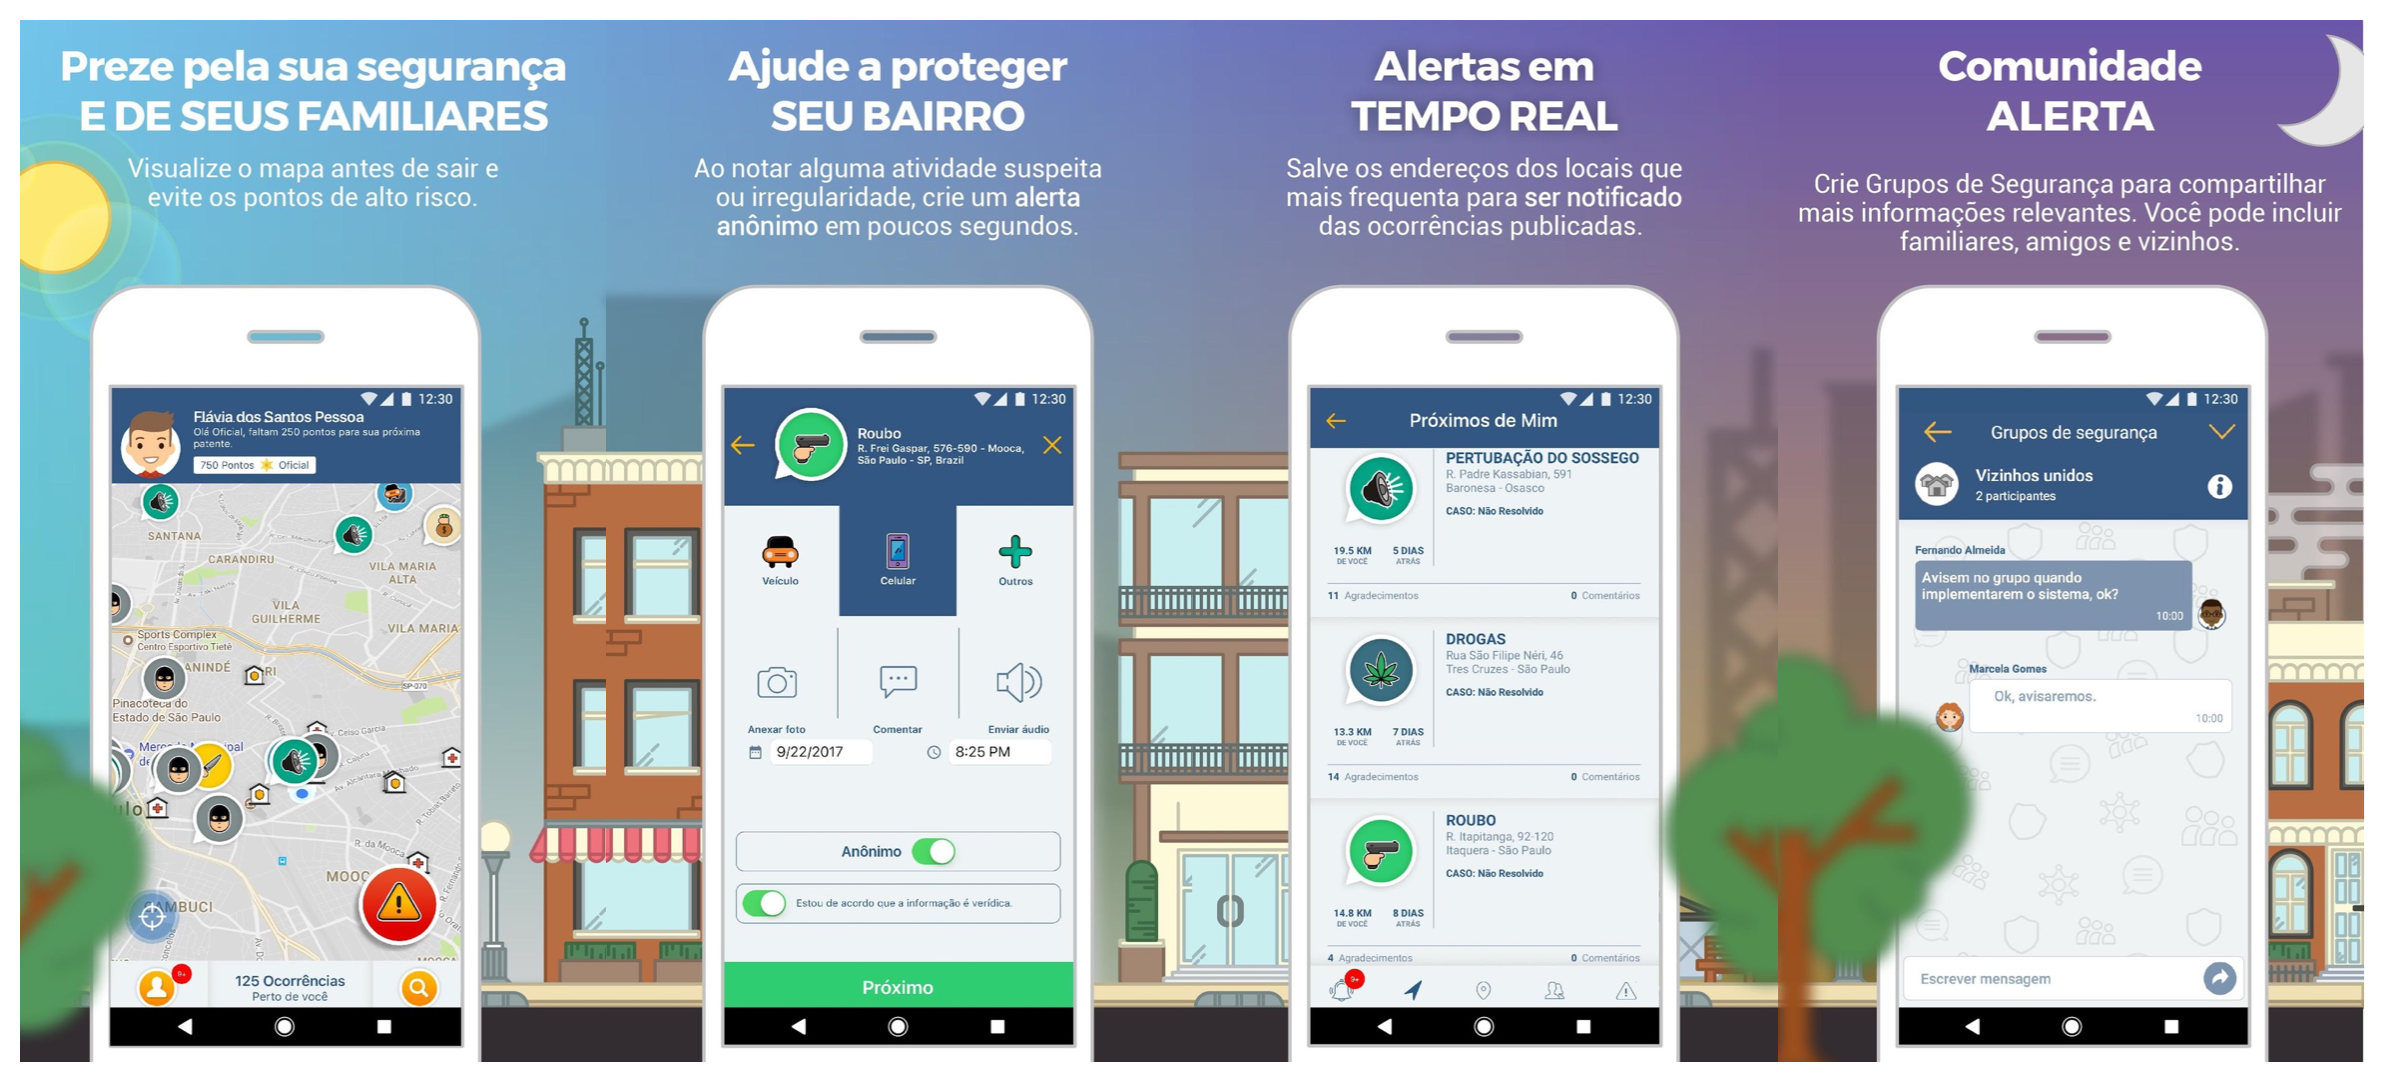
\includegraphics[width=\textwidth]{./images/sp-mais-segura.png}
	\label{f.sp-mais-segura}
	\legend{\small Fonte: Google Play.}
\end{figure}

\subsection{Análise}
% - Ao final da seção deverá ser feita uma análise crítica das soluções existentes.
% - Como base nessa análise, os objetivos do projeto proposto deverão ser descritos de forma a caracterizar claramente suas diferenças em relação aos projetos existentes.

Dada as soluções existentes descritas, nota-se que o \emph{Citizen} é a maior referência do segmento no mundo. Porém, apesar de seu enorme sucesso, ele é restrito à apenas algumas cidades dos Estados Unidos e não apresenta previsão de expansão para o Brasil. O Brasil possui soluções para o problema, porém são limitadas, logo surgiu-se a oportunidade de oferecer uma solução alternativa.

\section{Objetivos}

% Esta especificação tem por objetivo definir em detalhes o trabalho que será desenvolvido na disciplina de TCC. Nessa fase, o aluno deve cumprir quatro objetivos fundamentais:

% a) Descrever claramente o problema que deseja resolver e sua motivação.  
% b) Pesquisar soluções existentes para o problema que deseja resolver.
% c) Propor uma solução alternativa para o problema, caracterizando as diferenças com as soluções existentes.
% d) Pesquisar as tecnologias e ferramentas que poderão ser utilizadas em seu projeto, a fim de avaliar sua viabilidade.

Este trabalho tem como objetivo apresentar o processo e as atividades para o desenvolvimento de uma aplicação móvel onde as pessoas possam se manter conscientes, em tempo real, de situações de perigo que eventualmente podem estar ocorrendo nas suas proximidades, como crimes, incêndios, ameaças, protestos, ruas interditadas, catástrofes naturais, entre outros. O aplicativo deve oferecer a infraestrutura para o desenvolvimento de um senso de comunidade. A integração dos alertas com os chamados das polícias locais não está incluso no escopo do projeto.

\chapter{Detalhamento do problema}

% - Nesta seção o problema e sua motivação devem ser apresentados em detalhes.
% - Devem ser caracterizados: 
% - a) A natureza do problema. 
% - b) A importância do problema: quais segmentos da sociedade são afetados por ele. 
% - c) O impacto econômico que o problema causa atualmente e os benefícios esperados com sua solução. 
% - d) Os requisitos, funcionais, de desempenho e de custo, que uma possível solução para o problema deverá satisfazer.

\section{Natureza do problema}

% TODO: citar fontes aqui do pq seguranca publica no brasil é problema
% TODO: trazer dados?
A segurança pública no Brasil é dever do Estado, porém o serviço oferecido não é eficiente. O Estado está distante do cotidiano do cidadão, o tempo de resposta dos chamados policiais muitas vezes não é rápido o bastante, entre outros.

Sendo assim, um ambiente online que ofereça a infraestrutura necessária para a construção de verdadeiras comunidades locais, onde a confiança é estabelecidade com o tempo, com a ajuda de vídeos e images dos alertas que forem reportados, pode ajudar a amenizar o problema.

\section{Requisitos}

Dado a natureza do problema, uma solução para o problema deve atender os requisitos listados.

\subsection{Requisitos funcionais}

\begin{alineas}
	\item Usuários devem ser capazes de se registrar e logar no sistema.
	\item Usuários devem ser capazes de publicar alertas, que devem suportar o upload de fotos e vídeos de curta duração;
 	\item Usuários devem ser capazes de visualizar um mapa com os alertas mais recentes das suas proximidades;
	\item Usuários devem ser notificados quando alertas forem publicados nas suas proximidades; e
	\item Usuários devem ser capazes de definir qual o raio de proximidade em que ele está interessado, em metros.
\end{alineas}

\subsection{Requisitos não funcionais}

\begin{alineas}
	\item o sistema deve ser seguro;
	% \item o sistema deve ser altamente disponível, e em virtude disso, é aceitável uma temporária inconsistência;
	\item o sistema deve ser altamente confiável, ou seja, qualquer foto ou vídeo carregado nunca deve ser perdido;
	\item os usuários do aplicativo devem ter uma experiência de uso em tempo real; e
	\item o sistema deve suportar uma alta carga de leituras com latência mínima, sendo tolerável uma latência maior em escritas.
\end{alineas}

\chapter{Descrição do sistema}

% - Caracterizar claramente o projeto em termos de suas funcionalidades e da forma de sua interação com o usuário e com o ambiente.
% - Apresentar um diagrama em blocos mostrando uma visão geral do sistema a ser desenvolvido.
% - Cada bloco (ou módulo) corresponde a uma representação lógica de uma parte da solução proposta, o qual realiza uma função identificável do sistema completo. Um bloco deve corresponder a uma parte do sistema que pode ser desenvolvida e testada de forma independente das demais.
% - Cada bloco deve será ser descrito individualmente, caracterizar suas entradas e saídas, o processamento que realiza e como se comunica com os demais blocos.
% - Deve ser indicado também, de maneira sucinta, como cada módulo será desenvolvido (se em hardware digital, hardware analógico, software em desktop, firmware embarcado, etc.).

O sistema como um todo segue uma arquitetura cliente-servidor, onde o usuário interage com uma aplicação cliente que, por sua vez, se comunica com um servidor através da internet utilizando algum protocolo de rede. A aplicação cliente, nesse caso, é um aplicativo para dispositivos móveis, enquanto o servidor é uma aplicação monolítica, ou seja, um serviço único que roda em um único processo. Foi considerado o desenvolvimento de vários microserviços, porém a arquiteture monolítica foi escolhida em virtude da simplicidade de desenvolvimento, facilidade de testes e de \emph{deploy}.

A Figura~\ref{f.system} ilustra os componentes físicos do sistema.

\begin{figure}[htbp]
	\caption{\small Componentes físicos do sistema.}
	\centering
	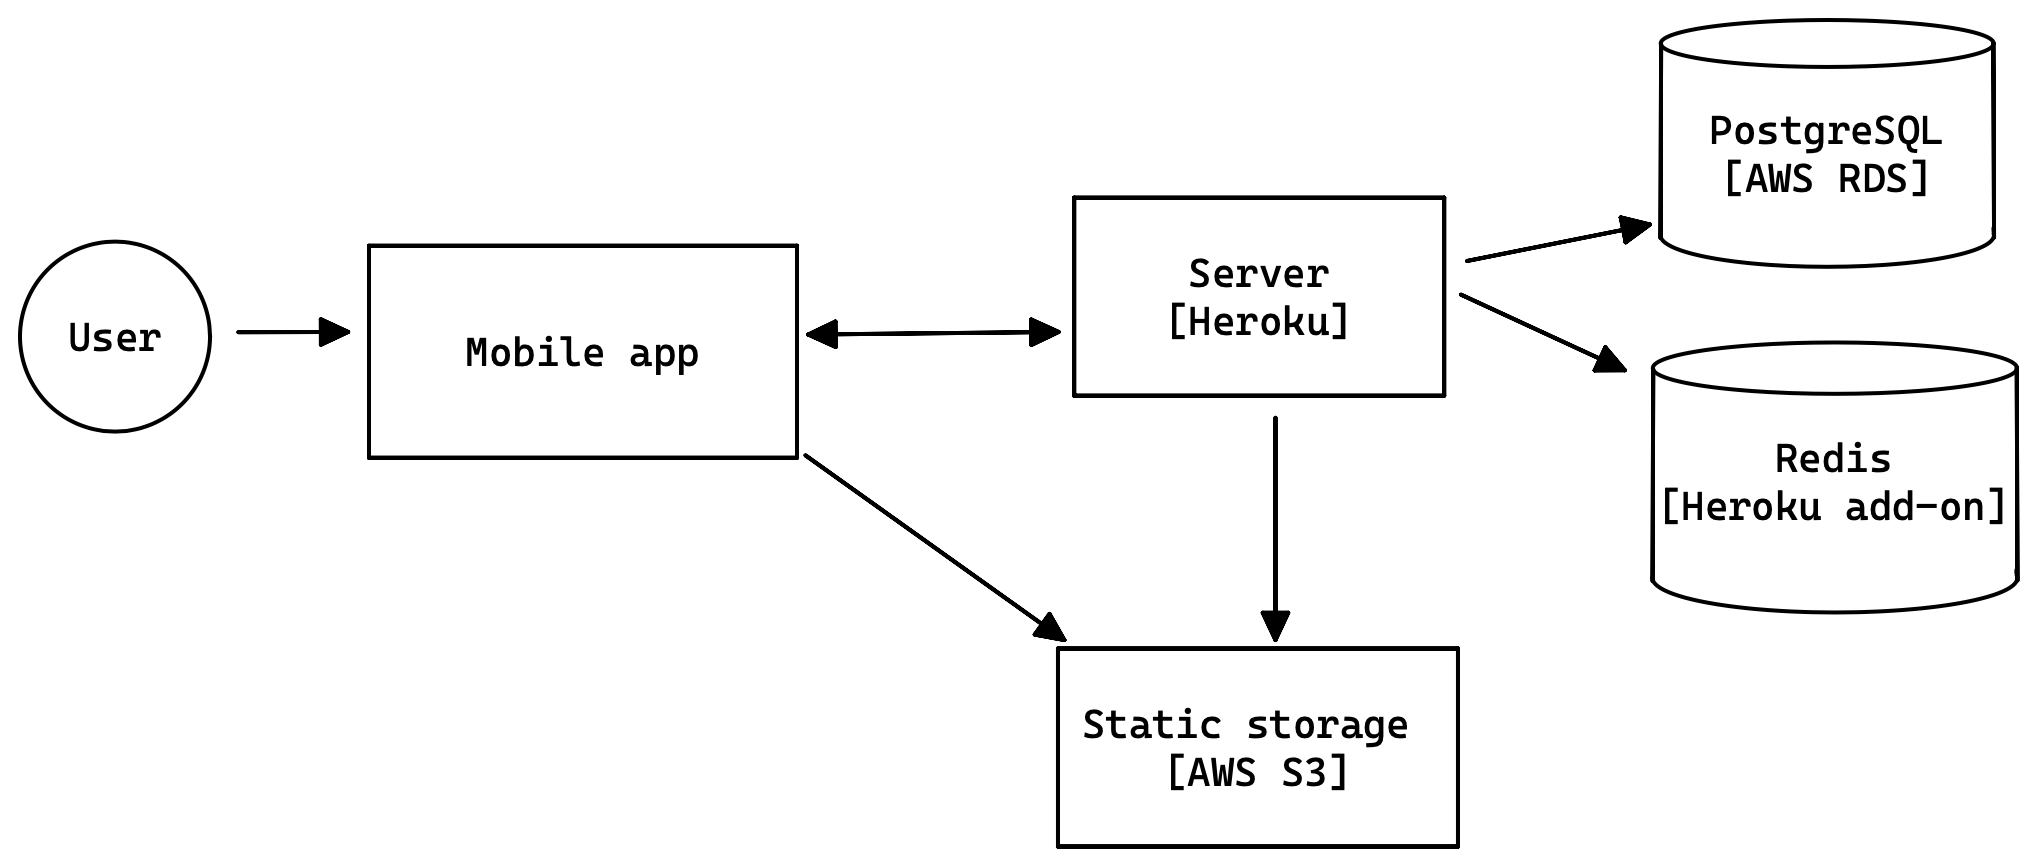
\includegraphics[width=\textwidth]{../diagrams/out/system.png}
	\label{f.system}
	\legend{\small Fonte: Elaborado pelo autor.}
\end{figure}

\FloatBarrier

\section{Servidor}

Os princípios do \emph{domain-driven design}, termo cunhado inicialmente por Eric Evans ~\cite{domain-driven-design}, e a ideias propostas por Uncle Bob em \emph{Clean Architecture} ~\cite{clean-architecture} tiveram grande contribuição para o projeto do servidor, tendo em vista que a \emph{separation of concerns} e a divisão da aplicação em camadas bem definidas com um rico modelo de domínio no centro permitem com que a complexidade do projeto cresça de forma manutenível ao longo do tempo.

A partir dos requisitos listados na Seção~\ref{s.requisitos}, se fez necessário identificar os diferentes subdomínios do sistema. Um módulo, também chamado de subdomínio, é um pedaço isolado de código. Como ilustrado pela Figura~\ref{f.system_server}, os seguintes módulos foram identificados:

\begin{itemize}
	\item \texttt{user module}: responsável pelos usuários, gerenciamento de identidade, autenticação e autorização;
	\item \texttt{incident module}: responsável por todas as operações relacionadas aos alertas;
	\item \texttt{notification module}: responsável pelo envio de notificações aos dispositivos dos usuários;
	\item \texttt{shared module}: módulo global para reuso de código entre diferentes módulos.
\end{itemize}

\begin{figure}[htbp]
	\caption{\small Visão geral do sistema.}
	\centering
	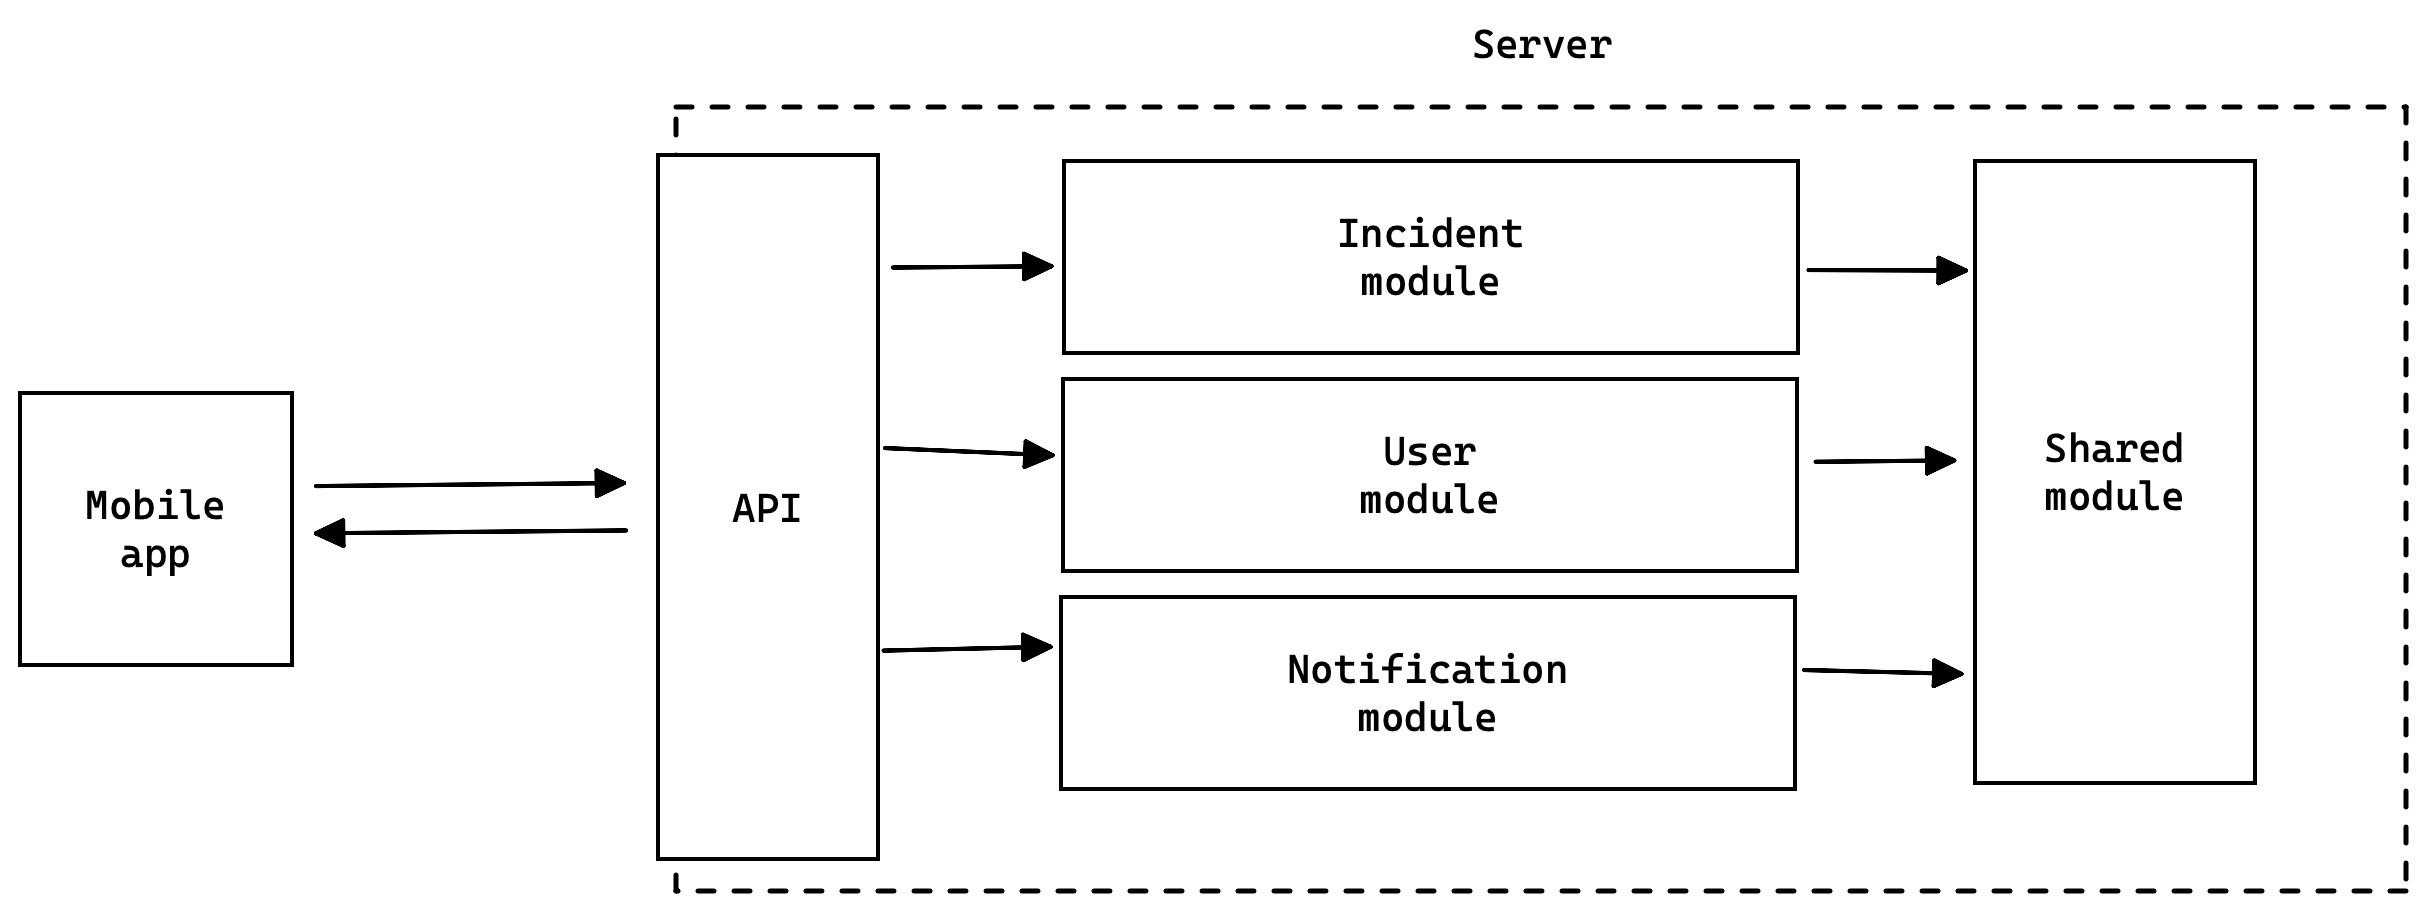
\includegraphics[width=\textwidth]{../diagrams/out/system_server.png}
	\label{f.system_server}
	\legend{\small Fonte: Elaborado pelo autor.}
\end{figure}

\FloatBarrier

\subsection{Camadas de cada módulo}

De acordo com a "arquitetura hexagonal" de Alistair Cockburn ~\cite{hexagonal-architecture}, a camada mais interna da arquitetura deve manter a camada de aplicação e domínio, e fora dessa camada devem estar os adaptadores (ou portas). Os adaptadores são "uma maneira de conectar o mundo exterior ao mundo interior". A aplicação é escrita em cima das tecnologias específicas que existem no "mundo exterior", como bancos de dados, APIs externas e serviços em nuvem. Definindo adaptadores, as tecnologias específicas podem ser envolvidos com segurança pela aplicação, o que é chamado de inversão de dependência. Esse tipo de arquitetura trás inúmeros benefícios como: 

\begin{alineas}
	\item Atrasar a decisão sobre exatamente qual tipo de servidor web, banco de dados, serviços externos ou tecnologia de cache será escolhido até que seja absolutamente necessário decidir. Facilitando, por exemplo, que se faça uma implementação inicial em memória do bancos de dados para agilizar o desenvolvimento;
	\item Prioriza a escrita de código que pode ser facilmente testado usando injeção de dependência, minimizando o uso de dependências concretas que poderiam tornar o código não testável; e
	\item Ajusta o foco às coisas específicas da aplicação e do domínio.
\end{alineas}

Portanto, cada um dos módulos respeita a divisão em camadas descrita pela Figura~\ref{f.system_server_each-module_layers}, onde camadas mais externas dependem das camadas mais internas e, consequentemente, camadas mais internas não conhecem camadas mais externas. 

\begin{figure}[htbp]
	\caption{\small Camadas de um módulo do servidor.}
	\centering
	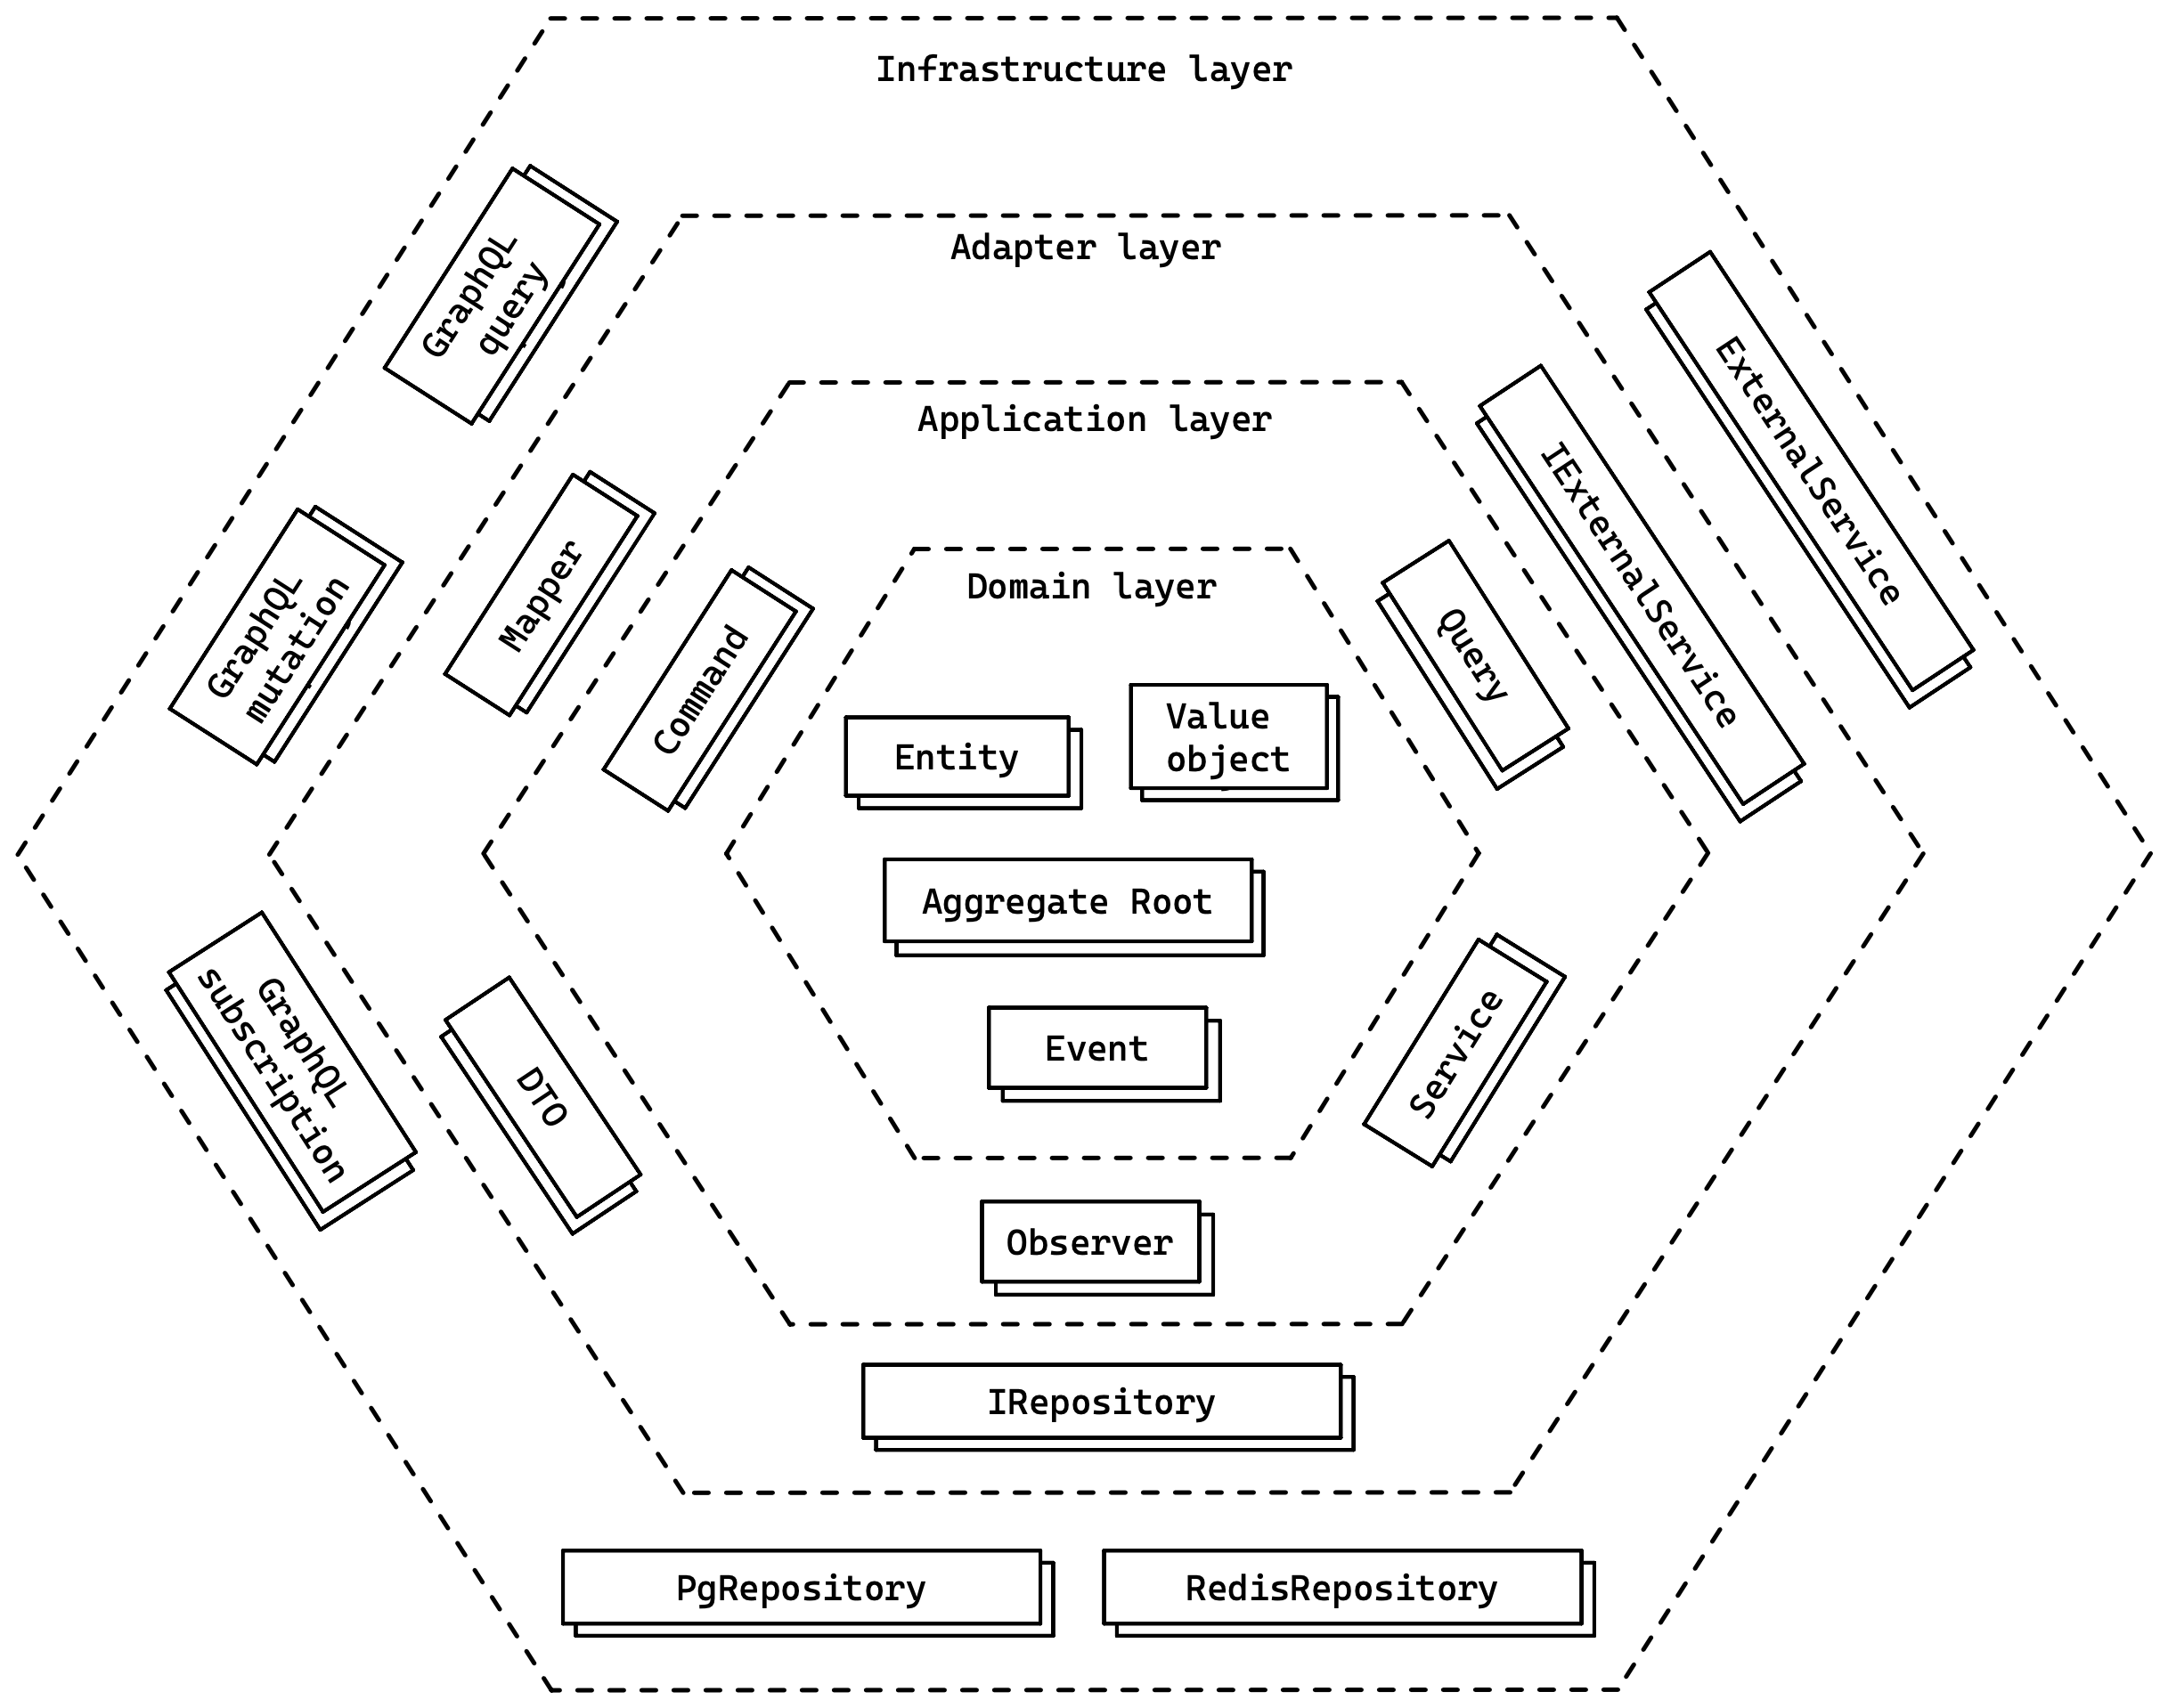
\includegraphics[width=\textwidth]{../diagrams/out/system_server_each-module_layers.png}
	\label{f.system_server_each-module_layers}
	\legend{\small Fonte: Elaborado pelo autor.}
\end{figure}

\FloatBarrier

\subsubsection{A camada de domínio}

A \texttt{domain layer} é a camada mais interna. É a camada que contém tudo aquilo que é importante para o negócio e que está menos propensa a mudar, configurando-se como a camada mais estável dentre todas e a qual todas as outras dependem.

Para encapsular regras de validação, existem os \texttt{value objecs}. Uma \texttt{entity} é um objeto que encorpa um pequeno conjunto de regras de negócio.

Um \texttt{aggregate root} é um tipo específico de \texttt{entity} que pode emitir \texttt{domain events} quando algo relavante para o negócio ocorre, e para isso, ele armazena como estado os eventos que ainda não foram emitidos pela camada de infraestrutura. Ele é implementado pela principal entidade de um \emph{cluster} de \texttt{entities} e \texttt{value objects} relacionados, os quais são tratados como uma única unidade de mudança.

A Figura~\ref{f.system_server_shared-module_domain} demonstra como essas classes abstratas são definidas no módulo \texttt{shared}, além da implementação da classe \texttt{DomainEvents}.

\begin{figure}[htbp]
	\caption{\small Diagrama de classes da camada de domínio do módulo compartilhado do servidor.}
	\centering
	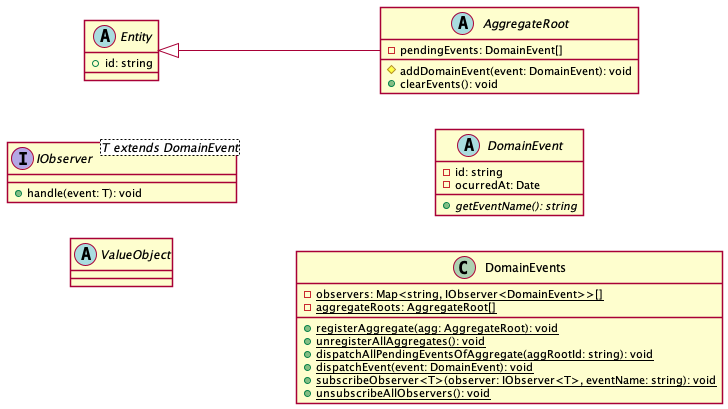
\includegraphics[width=\textwidth]{../diagrams/out/system_server_shared-module_domain.png}
	\label{f.system_server_shared-module_domain}
	\legend{\small Fonte: Elaborado pelo autor.}
\end{figure}

\FloatBarrier

A classe \texttt{DomainEvents} é um \emph{singleton}, ou seja, uma única instância global com tempo de vida vitalício em relação ao tempo de vida da aplicação. Ela é usada para encapsular o estado de quais \texttt{observers} estão interessados em ouvir pelos eventos emitidos por determinados \texttt{aggregate roots}. As instâncias dos \texttt{aggregate roots} inscritos contém \texttt{domain events} que serão dispachados para seus \texttt{observers} quando a camada de infraestrutura persistir as alterações feitas.

\subsubsection{A camada de aplicação}

A \texttt{application layer} contém os casos de uso, ou seja, principais funcionalidades, da aplicação. Em relação ao ambiente externo as entradas são os \texttt{commands} e \texttt{queries}, mas essa camada também implementa \texttt{application services} e \texttt{observers}, que são funções que serão executadas quando um determinado evento de domínio ocorre.

O \emph{Command-Query Separation (CQS)} é um padrão introduzido por Bertrand Meyer ~\cite{object-oriented-software-construction} que afirma que um método é ou um \texttt{command} que executa uma ação ou uma \texttt{query} que retorna dados ao chamador, mas nunca ambos. Dessa forma os fluxos de operações que mudam o sistema (e geram efeitos colaterais) são separados daqueles que apenas requisitam dados ao sistema, tornando o código mais simples de entender e manter.

\subsubsection{A camada de adaptadores}

A \texttt{adapter layer} contém abstrações para que a \texttt{application layer} possa interagir com a \texttt{infrastructure layer} sem depender dela, habilitando o que é chamado de inversão de dependência. Interfaces de repositórios que acessam bancos de dados, interfaces ou classes abstratadas que chamam APIs externas e mapeadores de objetos entre diferentes camadas (modelo de domínio, DTO, modelo de persistência) são exemplos do que pode estar nessa camada..

\subsubsection{A camada de infraestrutura}

A \texttt{infrastructure layer} é a camada mais externa. Ela contém os detalhes da aplicação, os quais possuem maior chance de serem trocados por outras bibliotecas ou frameworks específicos ao decorrer do tempo. Isso inclui implementações concretas das abstrações definidas na \texttt{adapter layer} para que elas possam ser executadas em \emph{runtime}, como serviços externos, repositórios para acesso à bancos de dados. Além disso, também contém lógicas de apresentação, como \texttt{HTTP endpoints} e \texttt{GraphQL operations}.

\subsection{Módulos}

Na sequência tem-se uma visão mais ampla de todos os módulos e como eles se inter-relacionam. Um módulo apenas deve se comunicar com outro via eventos de domínio, permitindo o desacoplamento entre eles.

A Figura~\ref{f.system_server_all-modules_domain-entities} ilustra como as entidades de cada módulo estão definidas. 

\begin{figure}[htbp]
	\caption{\small Entidades de domínio de cada módulo do servidor.}
	\centering
	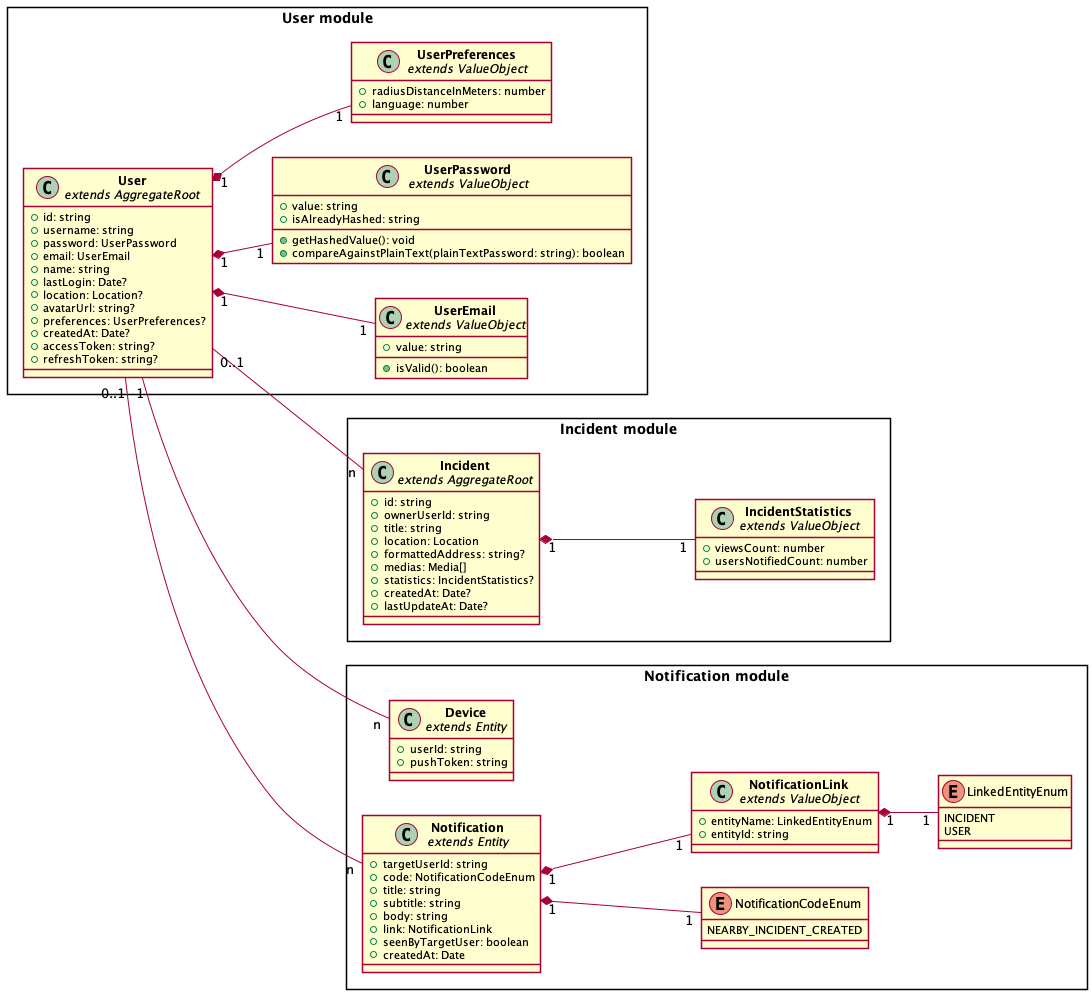
\includegraphics[width=\textwidth]{../diagrams/out/system_server_all-modules_domain-entities.png}
	\label{f.system_server_all-modules_domain-entities}
	\legend{\small Fonte: Elaborado pelo autor.}
\end{figure}

\FloatBarrier

A Figura~\ref{f.system_server_all_modules_commands-observers-events} ilustra as entradas e saídas de cada módulo.

\begin{figure}[htbp]
	\caption{\small Entradas e saídas de cada módulo do servidor.}
	\centering
	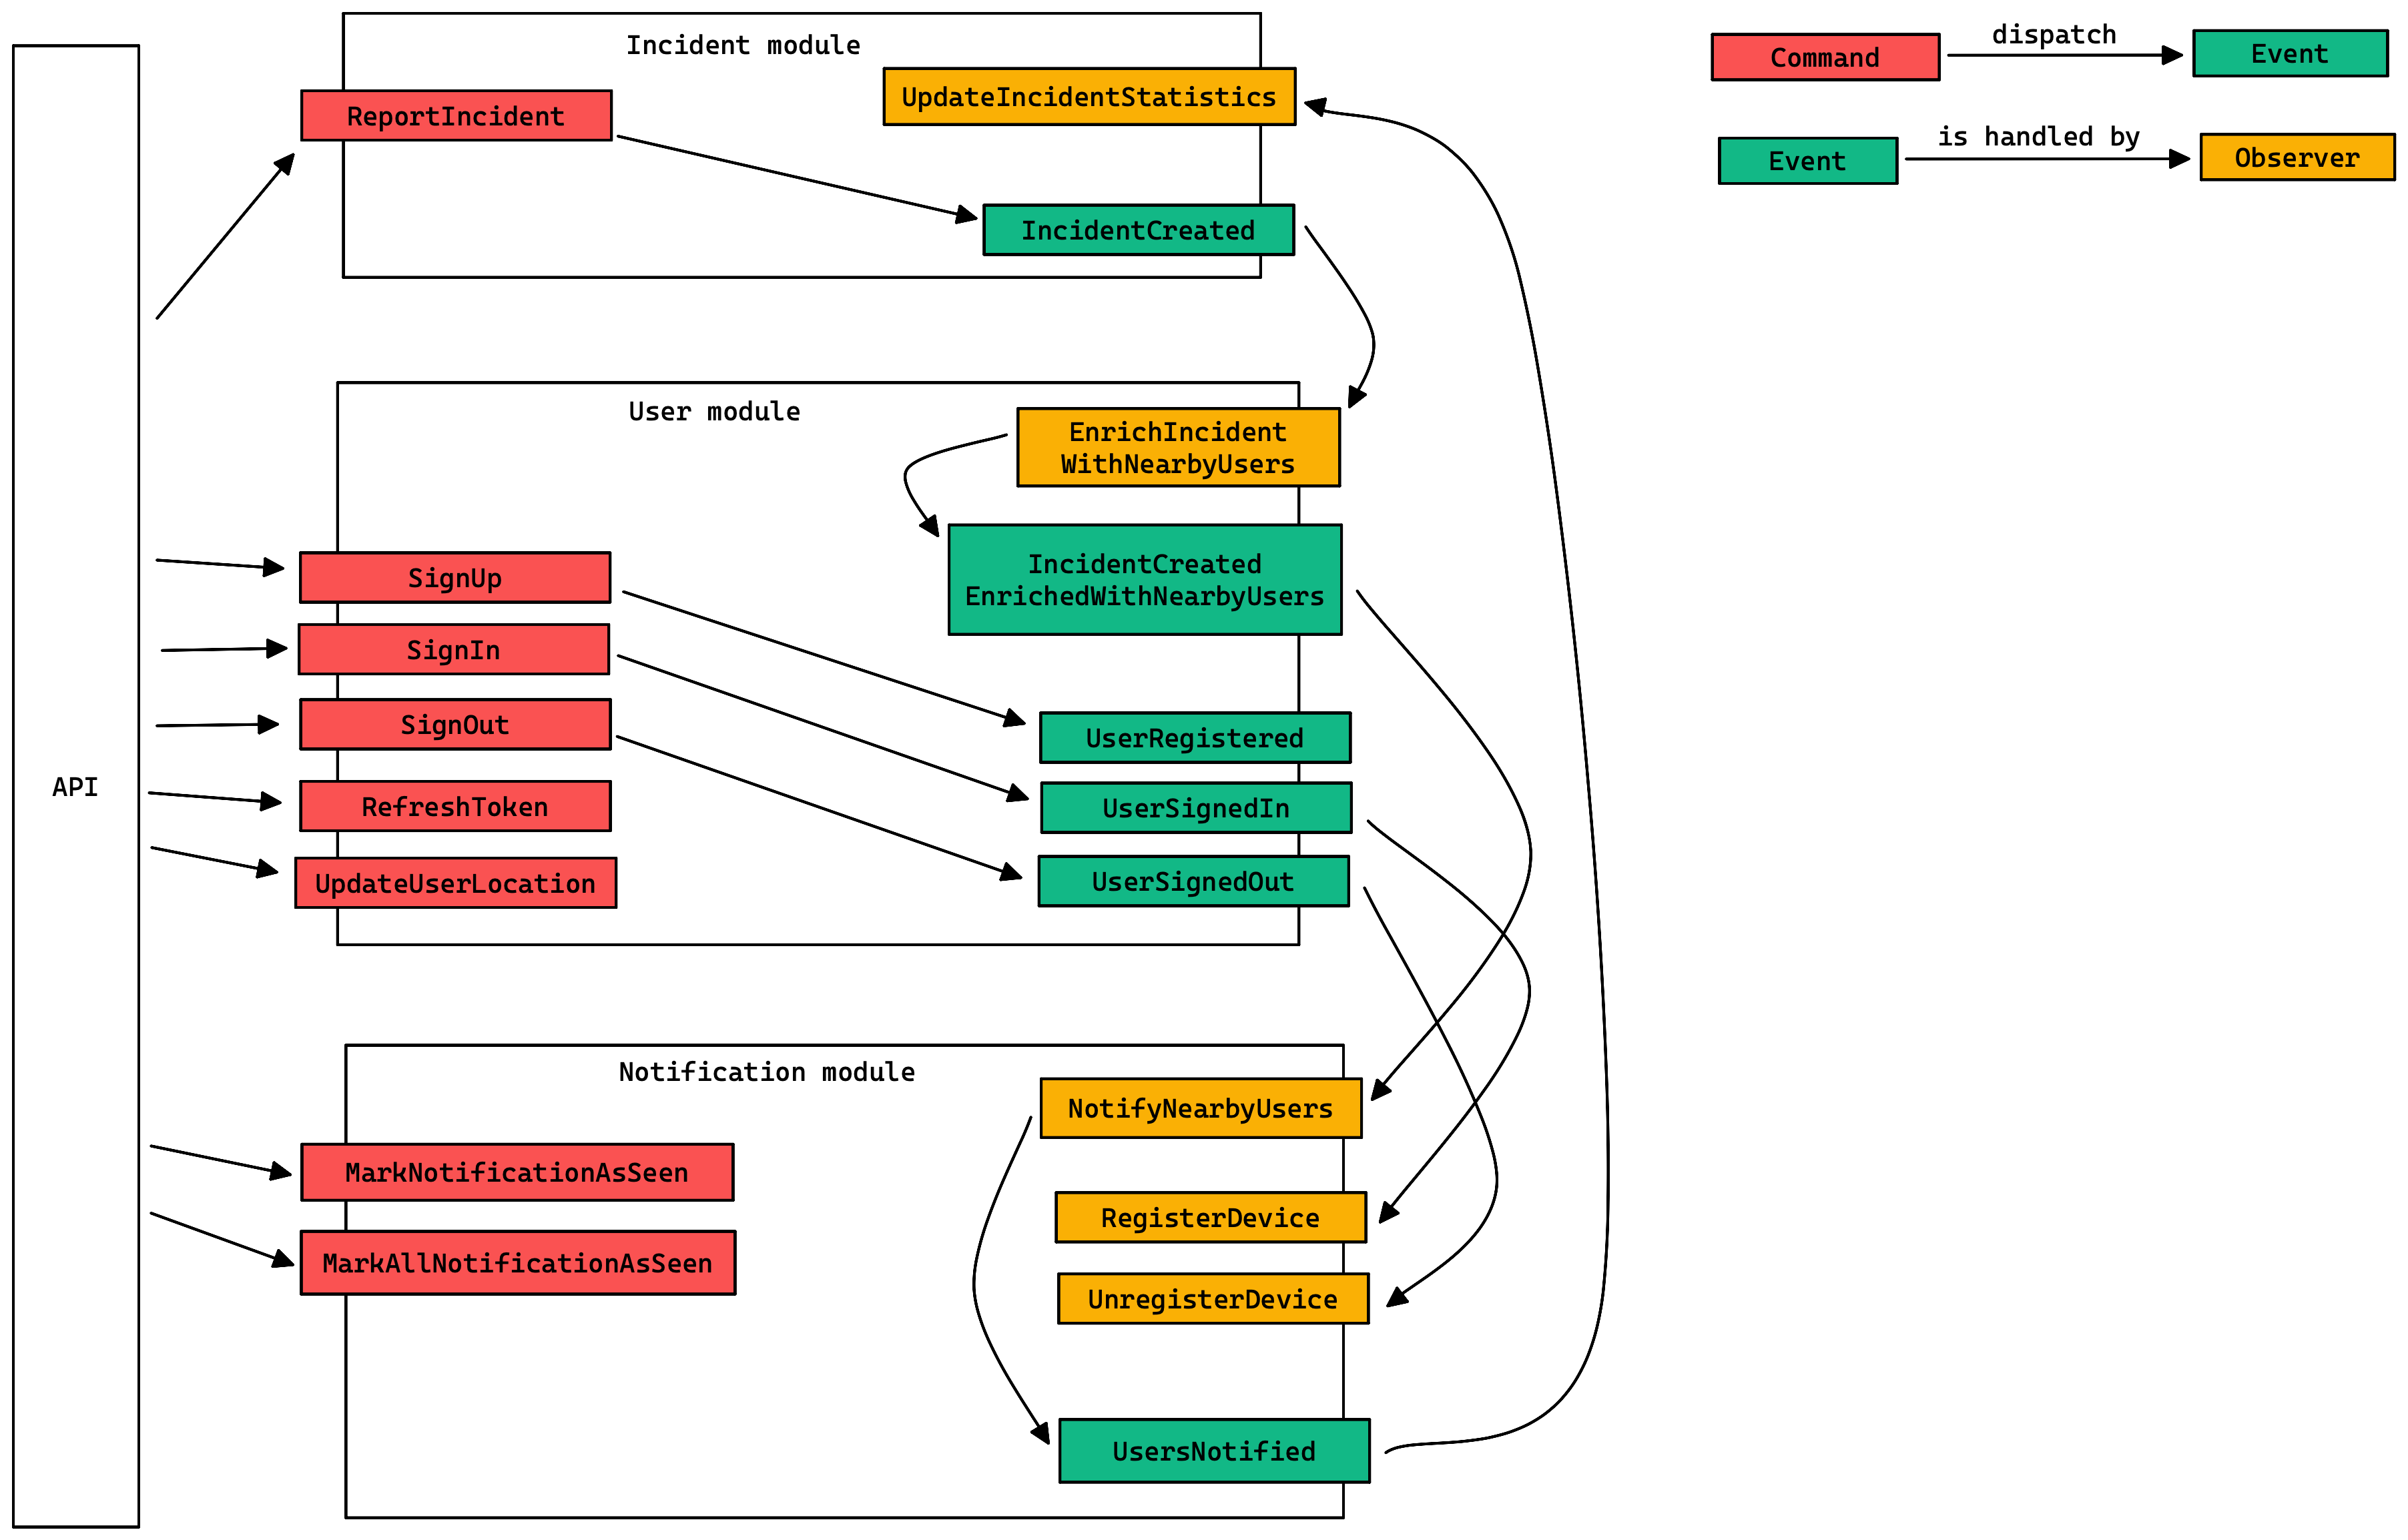
\includegraphics[width=\textwidth]{../diagrams/out/system_server_all_modules_commands-observers-events.png}
	\label{f.system_server_all_modules_commands-observers-events}
	\legend{\small Fonte: Elaborado pelo autor.}
\end{figure}

\FloatBarrier

\subsection{Principais tecnologias} % TODO

Para a implementação do servidor, tecnologias específicas foram escolhidas e cada uma delas tiveram um motivador de escolha.

% \paragraph{Node.js}

% O node~\cite{node}
% Por que Node?

% \paragraph{Redis}
% Por que Redis?

% \paragraph{PostgreSQL}
% Por que PostgreSQL?

\section{Comunicação entre servidor e cliente}

\subsection{GraphQL}
% vatangens do GraphQL: https://khalilstemmler.com/articles/graphql/graphql-architectural-advantages/#The-Data-Graph

GraphQL~\cite{graphql} é uma linguagem de consulta para APIs que permite com que clientes requisitem e recebam do servidor exatamente os dados que eles precisam. Ele possui seu próprio sistema de tipos e campos, ao contrário de \emph{endpoints} de um tradicional servidor HTTP que segue princípios REST.

Para criar uma API GraphQL é necessário instalar uma biblioteca que o implementa as especificações do GraphQL  na linguagem desejada, expor um endpoint para receber as requisições GraphQL, definir um \texttt{GraphQL schema} e conectar os \texttt{resolvers} de cada campo aos seus respectivos \texttt{data sources}.

O \texttt{GraphQL schema} é definido em um arquivo declarativo e auto-documentável. Ele é conhecido tanto pelo servidor como pelo cliente e atua como uma camada virtual entre eles. Ele define um grafo com todos os dados que o servidor está expondo, assim como todas as operações disponíveis para a busca e alteração desses dados. Os dados que estão sendo expostos para consultas são definidos através de \texttt{GraphQL queries}, já os que estão sendo expostos para serem alterados, através de \texttt{GraphQL mutations}. Além deles, também existem as \texttt{GraphQL subscriptions}, usadas quando o cliente deseja ouvir por atualizações do servidor. Todos eles, juntos, são chamados de \texttt{GraphQL operations}.

\subsection{Do cliente ao módulo do servidor}

A Figura~\ref{f.system_server_api} ilustra de forma mais detalhada como o aplicativo se comunica com o servidor. Para \texttt{GraphQL queries} e \texttt{GraphQL mutations} há um fluxo síncrono de requisição-resposta onde é utilizado o protocolo HTTP, enquanto que para \texttt{GraphQL subscriptions} há um fluxo assíncrono e onde é estabelecida uma conexão persistente via o protocolo WebSocket para que o servidor possa também enviar atualizações ao cliente sem que haja uma requisição prévia feita dele. Isso permite com que o usuário visualize os dados mais atualizados possíveis na tela. Alertas criados próximo à um usuário que está com o aplicativo aberto é um exemplo de atualização enviada apenas pelo servidor através de uma \texttt{GraphQL subscription}, a qual a aplicação cliente fica ``ouvindo'' desde o momento em que é iniciada.

\begin{figure}[htbp]
	\caption{\small Interação detalhada entre cliente e servidor.}
	\centering
	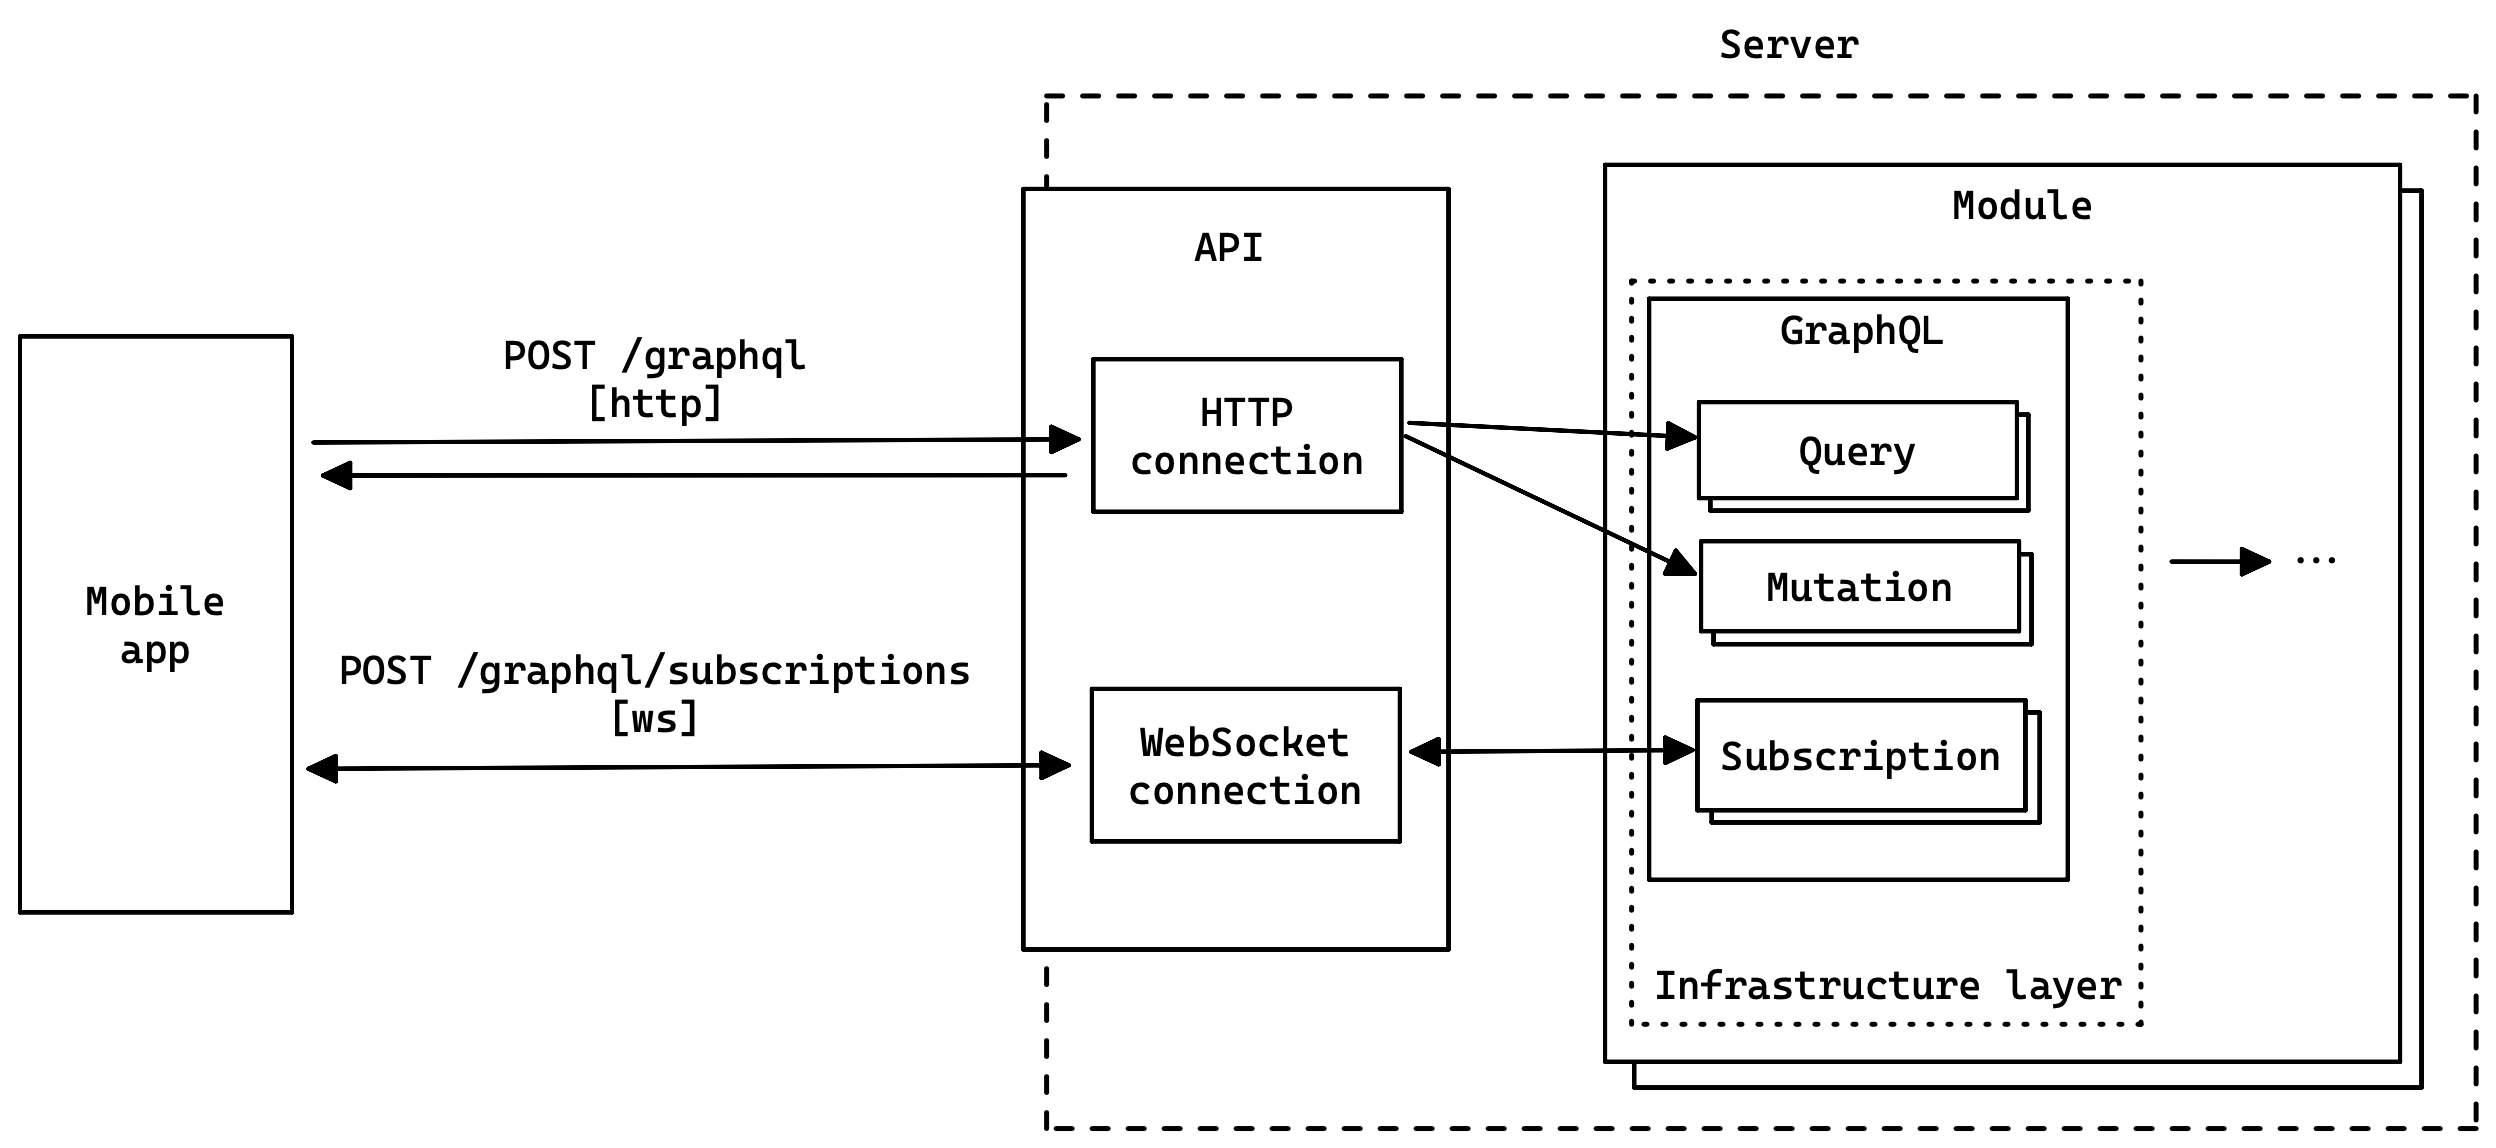
\includegraphics[width=\textwidth]{../diagrams/out/system_server_api.png}
	\label{f.system_server_api}
	\legend{\small Fonte: Elaborado pelo autor.}
\end{figure}

\FloatBarrier

\section{Aplicativo} % TODO

% TODO: diagram com: relay cache, graphql subscriptions, background location tracker, notifications listener

% TODO: permissoes com SO exigidas

% TODO: print das telas

\subsection{Principais tecnologias}

\subsubsection{React Native}
% TODO: Por que React Native?

\subsubsection{Relay}
% TODO: Por que React Native?

\subsubsection{Print das telas}


\chapter{Conclusão}

Conclui-se que os requisitos funcionais e não funcionais do sistema foram atentidos. O usuário final é capaz de realizar as principais funções de negócio, como publicar alertas e ser notificado por novos alertas nas suas proximidades. A implementação de cada nova funcionalidade do sistema ocorreu de forma intercalada entre o servidor e o aplicativo. A adoção do framework Relay~\cite{relay} gerou uma alta curva de aprendizagem inicial, ma foi compensada pelo ganhos em performance, flexibilidade e escalabilidade do aplicativo.

Em relação à validação do servidor, conclui-se que ele foi testado localmente repetidas vezes durante o processo de desenvolvimento com a ajuda do Docker~\cite{docker} para provisionamento local dos banco de dados Redis e PostgreSQL. Cada módulo do servidor foi testado com testes unitários, ou seja, testes automatizados que devem testar uma única unidade de código e que devem ignorar dependências externas. O aplicativo foi testado de forma manual e em um ambiente local.

Ainda existem, porém, dúvidas em relação à receptividade da opinião público ao projeto. Como o aplicativo não foi distribuido em lojas em razão dos custos e por se tratar, ainda, de um projeto prematuro, a ideia não foi testada com usuários reais. Considerando que o problema atacado - a segurança - é sensível a todos e a solução envolve a confiança entre pessoas anônimas, o maior desafio transcende as barreiras tecnológicas e está relacionado ao ser humano. O usuário pode, por exemplo, usar o aplicativo de forma não moderada ao agir como um ``vigilante'', ``reporter criminal'' ou até mesmo como um ``justiçeiro''. Ele pode fornecer alertas equivocados, difamatórios, racistas ou mentirosos, sejam eles mal intencionados ou não.

O uso frequente do aplicativo pode levantar questões mais filosóficas aos usuários como: ``É melhor ser totalmente informado de todos os crimes e emergências e ficar possivelmente paranoico, ou ser totalmente ignorante deles mas viver em constante perigo?''


% --------------------------------------------------------
% ELEMENTOS PÓS-TEXTUAIS
% --------------------------------------------------------

\postextual


% --------------------------------------------------------
% REFERÊNCIAS BIBLIOGRÁFICAS
% --------------------------------------------------------

\bibliography{chapters/referencias}


% --------------------------------------------------------
% GLOSSÁRIO
% --------------------------------------------------------

% Consulte o manual da classe abntex2 para orientações sobre o glossário.
%\glossary


% --------------------------------------------------------
% APÊNDICES
% --------------------------------------------------------

% Inicia os apêndices
%\begin{apendicesenv}
% Imprime uma página indicando o início dos apêndices
%\partapendices
% Criação do apêndice
%\end{apendicesenv}


% --------------------------------------------------------
% ÍNDICE REMISSIVO
% --------------------------------------------------------

%\printindex


% --------------------------------------------------------
% FINAL DO DOCUMENTO
% --------------------------------------------------------

\end{document}
